\clearpage
\thispagestyle{empty}
~\clearpage
%\graphicspath{{Figures_chapter-2/}}
\chapter{Working of HackIT}
\label{chap2}
%\pagenumbering{arabic}

\section{Introduction}\label{2}
HackIT is a generic framework for cybersecurity tasks to study human learning and decision-making of hackers and analysts. It represents a simplified framework containing the most essential elements for creating cybersecurity scenarios: network nodes, which represents the characteristics of real nodes; strategies, which can be configured for creating deception; and commands, which are used for communication with the network. The analyst’s goal in the HackIT task is to evaluate different deception strategies and the hacker’s goal to identify the real network nodes and exploit them. Hackers communicate with the network in HackIT using different commands and gain information about different configurations. However, hackers are not aware of the strategies used by analysts inside the HackIT scenario. Hackers basically learn about these strategies overtime by playing different rounds. Thus, HackIT is a controllable and flexible simulation tool with the capability of creating various network scenarios and experiment with different techniques to lure hackers.

Previously HackIT tool was available for creating deception with limited number of systems only and for single player games only. In our project, we implemented the enhanced capabilities of HackIT tool. Specifically, our implementation would make the the HackIT tool capable of running experiments with different sized networks, different network configurations, different deception strategies, and single player and multiplayer games. Thus, the enhanced capabilities of HackIT tool can help us answer several questions such as the effect of different network sizes and honeypot allocations on hacker’s performance and the most effective way to present the “clues” of deception in network nodes.Specific characteristics of
HackIT tool added by our team are explained in the upcoming sections.
\section{Dynamic size of the Network}
The HackIT tool is flexible to create any number of nodes in the simulated/virtual network. The configuration of these systems will also be dynamically created. Thus, this tool will allow researchers to build experiments with small, medium and large scaled networks as shown in \ref{fig:figure4}
\FloatBarrier
\begin{figure}[!htbp]
\centering
  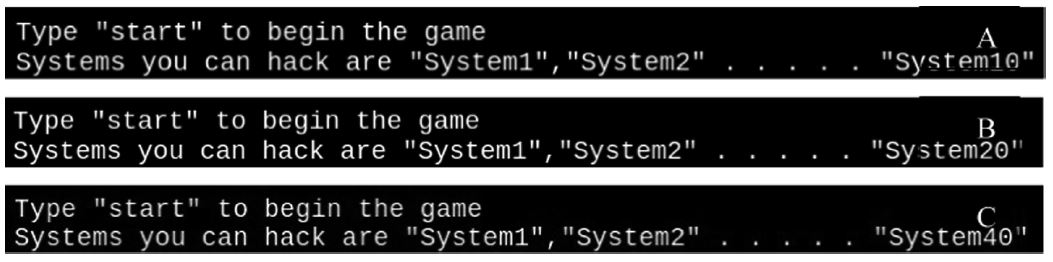
\includegraphics[scale=0.5]{Chap2/size.jpg}
  \caption{Network of Different Sizes: (A) 10 Systems (B) 20 Systems (C) 40 Systems}\label{fig:figure4}
\end{figure}     
\section{Allocation of Honeypots and Regular Computers}
The HackIT tool is capable of creating any proportion of network computers as honeypots. This tools also provides a functionality to define the features of honeypot that make them pretend as real systems. These features include the ability to configure vulnerable ports, vulnerable operating systems, and proportion of fake files on the honeypots. Thus, setting different proportion of honeypots and defining deception via honeypots is relatively easy in the new version of HackIT.
\section{Configuration of Computers}
The configuration of honeypots and regular computers is automatically generated by a script in HackIT that would produce the configuration for a fixed number of systems with a given proportion of honeypots and real systems. This script generates the configuration consisting of real systems, honeypots, and files for each game round in HackIT. By using this script, one could generate data onetime and encode it in the experiment so that it would present all participants with same configuration. For example, the regular systems could be configured as patched and difficult to exploit and honeypot systems could be configured as easy to exploit. This configuration mapping is shown in \ref{fig:figure3}.

\section{Content of Honeypots}
HackIT tool provide a facility to create fictitious content on honeypots using fake files. The proportion of fake files and useful files on a honeypot can be configured in HackIT. Figure \ref{fig:figure5} shows the output of the ls command in the directory where only pin.txt is a real file and rest are fake files. In HackIT tool, the number of files on each server can be dynamically created. We tested our platform with the different number of files ranging from 50\textendash200.
\FloatBarrier
\begin{figure}[!htbp]
\centering
  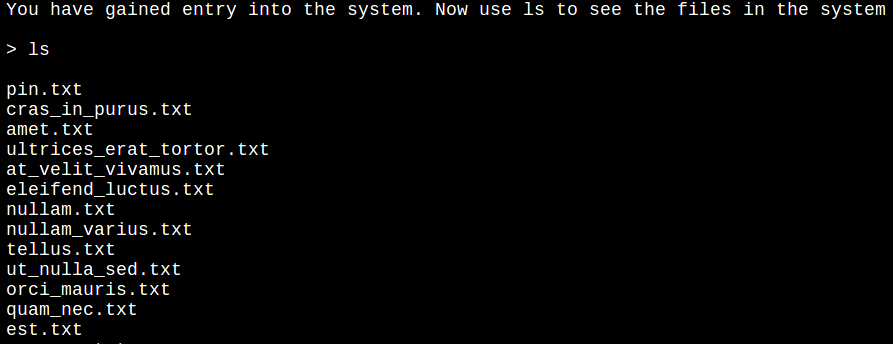
\includegraphics[scale=0.5]{Chap2/files.png}
  \caption{List of fake files on Honeypot webserver}\label{fig:figure5}
\end{figure} 
\section{Single-Player and Multi-Player Platform}
HackIT tool provides a functionality to run single-player and multi-player experiments.
In single-player experiment settings, players cannot communicate with each other.However, in multi-player experiment setup, players are provided with a chat functionality to share their knowledge. Hackers usually penetrate into the network by
organizing themselves into a group. Hackers in a group rely on information gained
from fellow hackers who have already penetrated into the network or are trying to
penetrate it Fig. \ref{fig:figure6}.
\FloatBarrier
\begin{figure}[!htbp]
\centering
  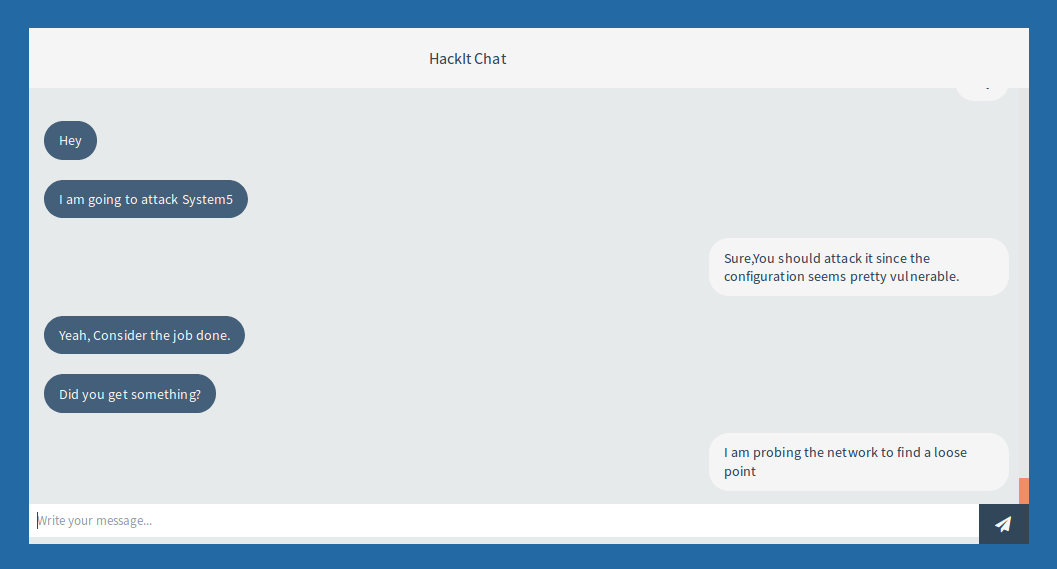
\includegraphics[scale=0.4]{Chap2/chat.png}
  \caption{Chat functionality for multiplayer experiments in HackIT}\label{fig:figure6}
\end{figure} 

\section{Commands}
The HackIT tool can run various network commands that include: nmap, use\_exploit, ls, and scp. Nmap is a network utility that shows the open ports, operating system type, and services running on the specified webserver. The nmap utility also provides the list of vulnerabilities on the corresponding webservers. The use\_exploit command exploits vulnerabilities of a system and helps attacker to gain access to a particular webserver. Next, the ls command lists the files currently on the file system of the machine. The scp command transfers files to the remote machine.
\section{Measures for Human-in-the-Loop Experiments}
For understanding the decision-making process of hackers, it is important to analyze how do they gather information, their preferences while searching for information, kind of exploits used, and most importantly how to they react to different defense strategies. HackIT tool provides various measures to analyze the human performance in cybersecurity experiments.

\begin{itemize}
    \item Probing behavior: HackIT tool provides capability to record the probing behavior of hacker participants. Probing is an important phase where hackers collect information before launching a real attack. Using deception in probing responses and analyzing hackers’ reaction towards deceptive responses is an important measure provided in HackIT tool.
    \item Attack behavior: HackIT measures the attack behavior of hackers by recording their attack actions, exploit information, their specific selection of targets or configuration. HackIT tool also records the vulnerabilities exploited, and exploits used by hackers. Defenders can analyze this data to study their attack patterns.
    \item Learning: HackIT tool can record overtime behavior of participants. Thus, it provides data to analyze learning capabilities of hackers against different deception strategies.
    \item Communication History: HackIT tool provides functionality to analyze the chatting history of hacker to investigate that how hackers make decisions or formulate strategies in team-based
    tasks.
    \item Time: HackIT tool also records time taken by hackers to exploit a system. Timing is another measure to evaluate the success of deception.
\end{itemize}
\clearpage 